\chapter{Arquitectura}
\label{chap:architecture}


\section{Introducción}
\label{sec:introduction}

En este capítulo trataremos la fase de diseño de este proyecto, así como los detalles de implementación de la arquitectura del mismo. Primero, presentaremos una vista general del proyecto por medio de un escenario. A continuación se mostrará la arquitectura en el cliente, así como la del servidor y los servicios que la componen. Posteriormente, se detallarán los módulos que conforman la aplicación, así como las métricas que se han decidido calcular y sus motivos. Con ello tenemos la intención de facilitar al lector una vista general de la arquitectura del proyecto.

Se presenta a continuación el escenario principal de uso de ChatStats:

\begin{figure}[H]
	\centering
	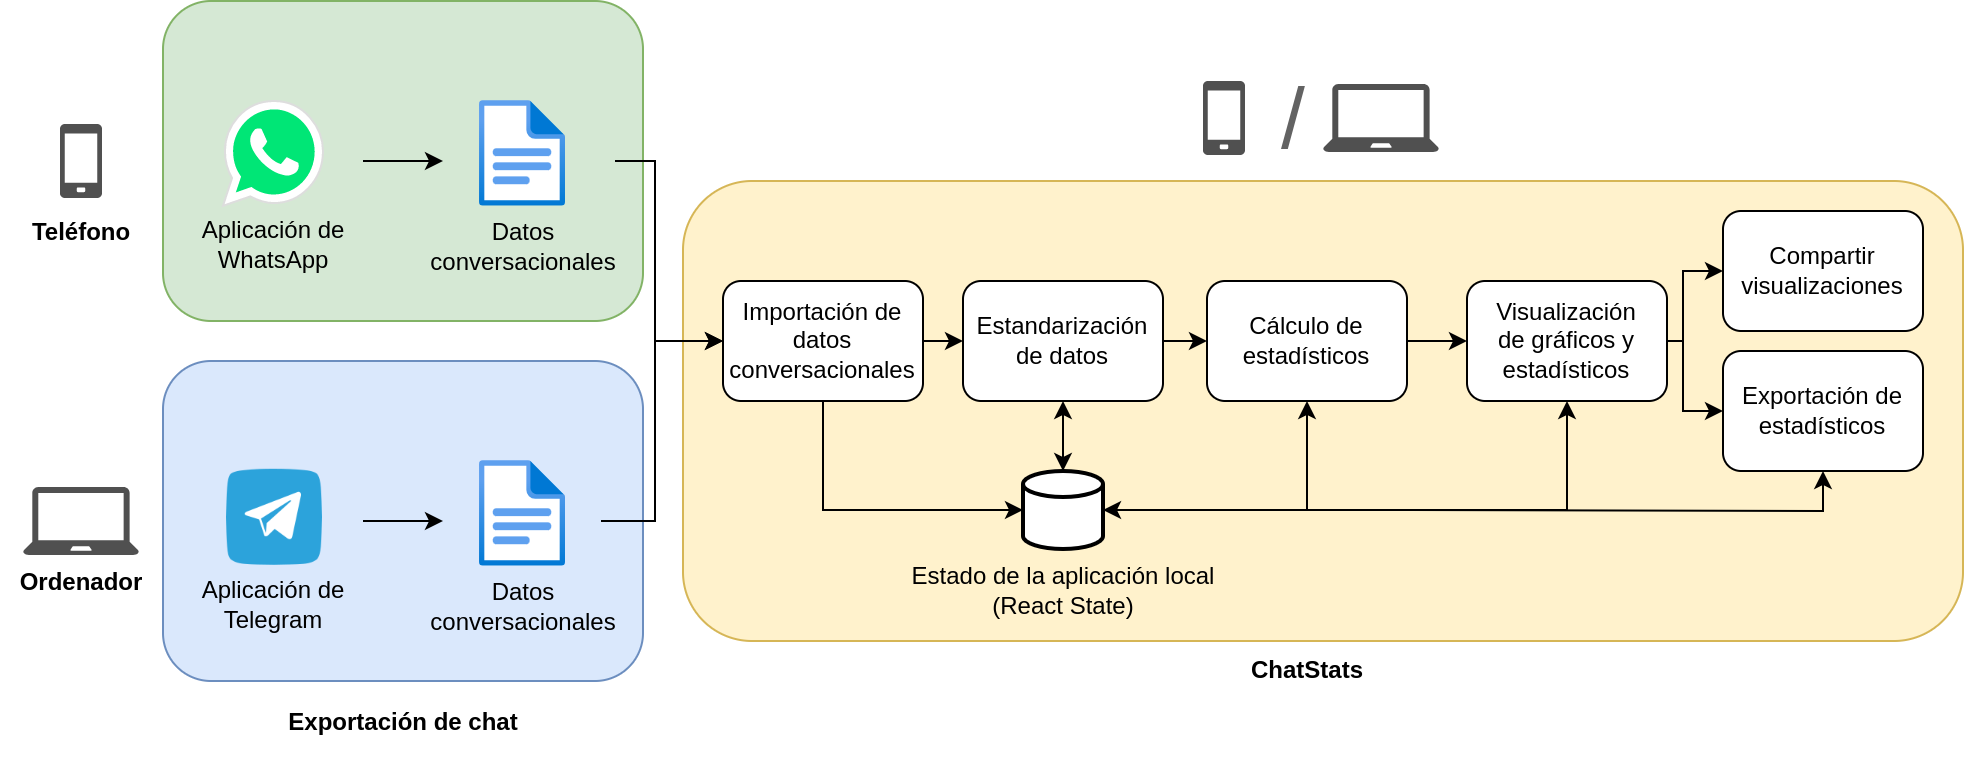
\includegraphics[width=\textwidth]{img/scenario.png}
	\caption{Escenario de ChatStats}
	\label{fig:chap4:architecture_scenario}
\end{figure}

\todi{El servidor únicamente sirve la página... ¿Debería meterlo aquí? ¿Cómo?}

Como se puede observar, el usuario debe exportar un chat desde la aplicación de WhatsApp (móvil) o Telegram para escritorio. Son estas las únicas versiones de las aplicaciones que permiten exportar las conversaciones. Con estos datos exportados, el usuario accede a ChatStats desde el navegador, ya sea en un dispositivo móvil o en un ordenador. El servidor le envía el cliente completo, por lo que no intercambia más peticiones en adelante. El usuario puede seleccionar e importar el archivo a la aplicación, que los estandariza, calcula métricas sobre la conversación y ofrece una visualización de los mismos. Finalmente, el usuario puede compartir las visualizaciones, así como exportar los datos calculados para su uso personal.


Se desarrolla toda la aplicación en \textit{JavaScript}, puesto que puede ejecutarse en todos los navegadores salvo que lo tengan deshabilitado. Otros lenguajes como \textit{PHP} o Python requieren de un servidor para realizar operaciones y que estos envíen una plantilla rellena con los resultados.



\section{Arquitectura en el cliente}

A continuación se presenta la arquitectura que podemos encontrar en un cliente cualquiera:

\begin{figure}[H]
	\centering
	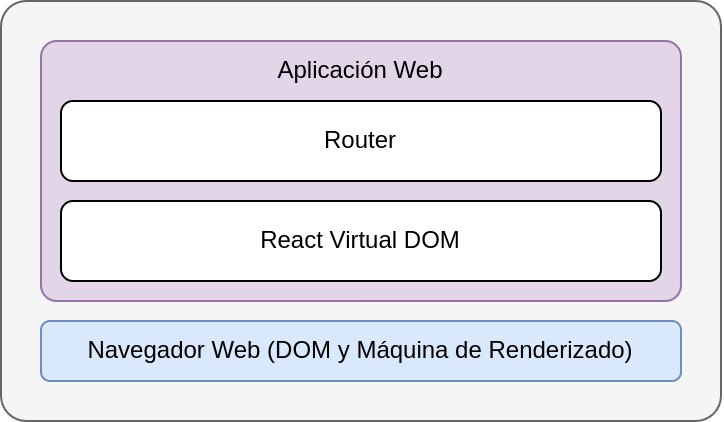
\includegraphics[width=0.6\textwidth]{img/client.png}
	\caption{Arquitectura en el cliente}
	\label{fig:chap4:architecture_client}
\end{figure}

\paragraph{Navegador.} El navegador juega un papel fundamental para el acceso y ejecución de cualquier aplicación web. Aunque no se entra en detalle en su estructura interna, sí que vamos a detallar la integración con \acrfull{pwa}. Esta integración que ofrecen algunos navegadores como los basados en Chromium, permite instalar aplicaciones web, con ventajas como:

\begin{itemize}
	\item La aplicación saldrá en el escritorio en teléfonos Android e iOS, así como en el cajón de aplicaciones del navegador.
	\item Posibilidad de acceso a notificaciones \textit{push} para el sistema (que no utilizaremos).
	\item Posibilidad de guardar en \textit{cache} el código del cliente, permitiendo su uso sin conexión a Internet.
\end{itemize}

Es por ello que ChatStats puede ser instalada en los dispositivos con navegador con soporte \acrshort{pwa}, permitiendo su instalación y ejecución sin acceso a Internet. Para ello, únicamente se debe registrar un \textit{service worker} que guarda el código en el cliente, así como un archivo de manifiesto que recoge un título, descripción e iconos de la aplicación.

Hay que mencionar también que Mozilla no ofrece soporte para \acrshort{pwa} en su navegador Firefox\cite{firefoxNoPWA}, aunque este puede ser habilitado mediante una extensión\cite{firefoxPWAextension}.

\paragraph{Aplicación Web.} Es la última capa, se encuentra nuestra aplicación, cuya arquitectura de procesamiento se explica en la \autoref{chap:architecture:processing}. Explicamos a continuación los componentes lógicos que se encuentran en el cliente:

\subparagraph{Router.} ChatStats es una aplicación multipágina. Esto quiere decir que cuenta con diferentes rutas web en las que se muestran diferentes páginas. La página principal consolida la ruta `\textit{/}', mientras que `\textit{/graphs}' enruta la página para la visualización de los gráficos.

\subparagraph{React Virtual DOM} El DOM virtual es un concepto de programación en el que una representación virtual de la interfaz de usuario (UI) es guardada en memoria y sincronizada con el DOM del navegador. Esto nos permite definir qué queremos en la interfaz de usuario y React conseguirá que el DOM virtual y el DOM del navegador se sincronicen.








\section{Arquitectura en el servidor}
\label{chap:architecture:server}

Se muestra a continuación una grafo de la arquitectura en el servidor, donde se muestran las capas que lo componen.

\begin{figure}[H]
	\centering
	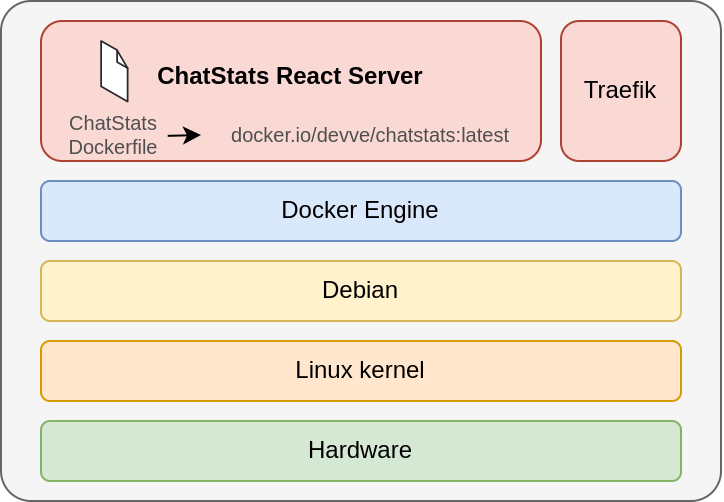
\includegraphics[width=0.6\textwidth]{img/server.png}
	\caption{Arquitectura en el servidor}
	\label{fig:chap4:architecture_server}
\end{figure}

Se ha decidido no instalar el software directamente sobre el sistema operativo, evitando problemas de dependencias y distintas versiones de las mismas para los componentes del sistema operativo. Asimismo, se evitan problemas de seguridad que puedan venir por vulnerabilidades en el código fuente y sus dependencias.

Hemos elegido virtualización ligera para ejecutar nuestro código en contenedores, por las razones que se exponen:

\begin{itemize}
	\item Se contienen las dependencias de terceros en una imagen.
	\item En caso de vulnerabilidad, solo se expone el contenedor y no el sistema completo.
	\item Los recursos se ocupan dinámicamente en función a las necesidades, al contrario que con la virtualización completa.
	\item Permite el despliegue en cualquier sistema operativo compatible con Linux, salvo arquitecturas ARM (que no es frecuente en servidores).
\end{itemize}

\paragraph{ChatStats React Server.} Se trata del servidor de React que sirve el contenido. Tras construir la versión de producción con el código fuente, este contenedor sirve el contenido estático final, que enviará al cliente completamente cuando este solicite la aplicación web. Se ha implementado por medio de un fichero Dockerfile, que parte de una imagen de \textit{NodeJS}, instala las dependencias y sirve el contenido. Con esta secuencia de instrucciones, se ha creado una imagen para uso en contenedores Docker, que puede encontrarse públicamente en el repositorio de imágenes DockerHub.

\paragraph{Traefik} Se ha decidido usar Traefik como \textit{proxy} inverso, que se sitúa frente al servidor de ChatStats para redirigir las peticiones realizadas a su contenedor correspondiente en el puerto adecuado.

Además, Traefik gestiona los certificados \acrshort{ssl} haciendo uso de \textit{Let's Encrypt}: autoridad sin ánimo de lucro que provee certificados para la capa \acrshort{tls} sin coste alguno.








\section{Arquitectura de la aplicación}
\label{chap:architecture:processing}


Con el objetivo de mantener la privacidad de los datos del usuario, se ha planteado una arquitectura centrada en el cliente, donde el servidor únicamente envía la totalidad de la aplicación al cliente en la primera petición. Esto supone un mayor coste computacional en el cliente para realizar todas las operaciones necesarias, por lo que la eficiencia del código es necesaria. Además, esta arquitectura se puede extender, en un futuro, ofreciendo analíticas adicionales si el usuario opta por enviar información al servidor para su procesamiento. Este caso de extensión se detallará más adelante.

A continuación se muestra la arquitectura de la lógica de negocio en la aplicación:

\begin{figure}[H]
	\centering
	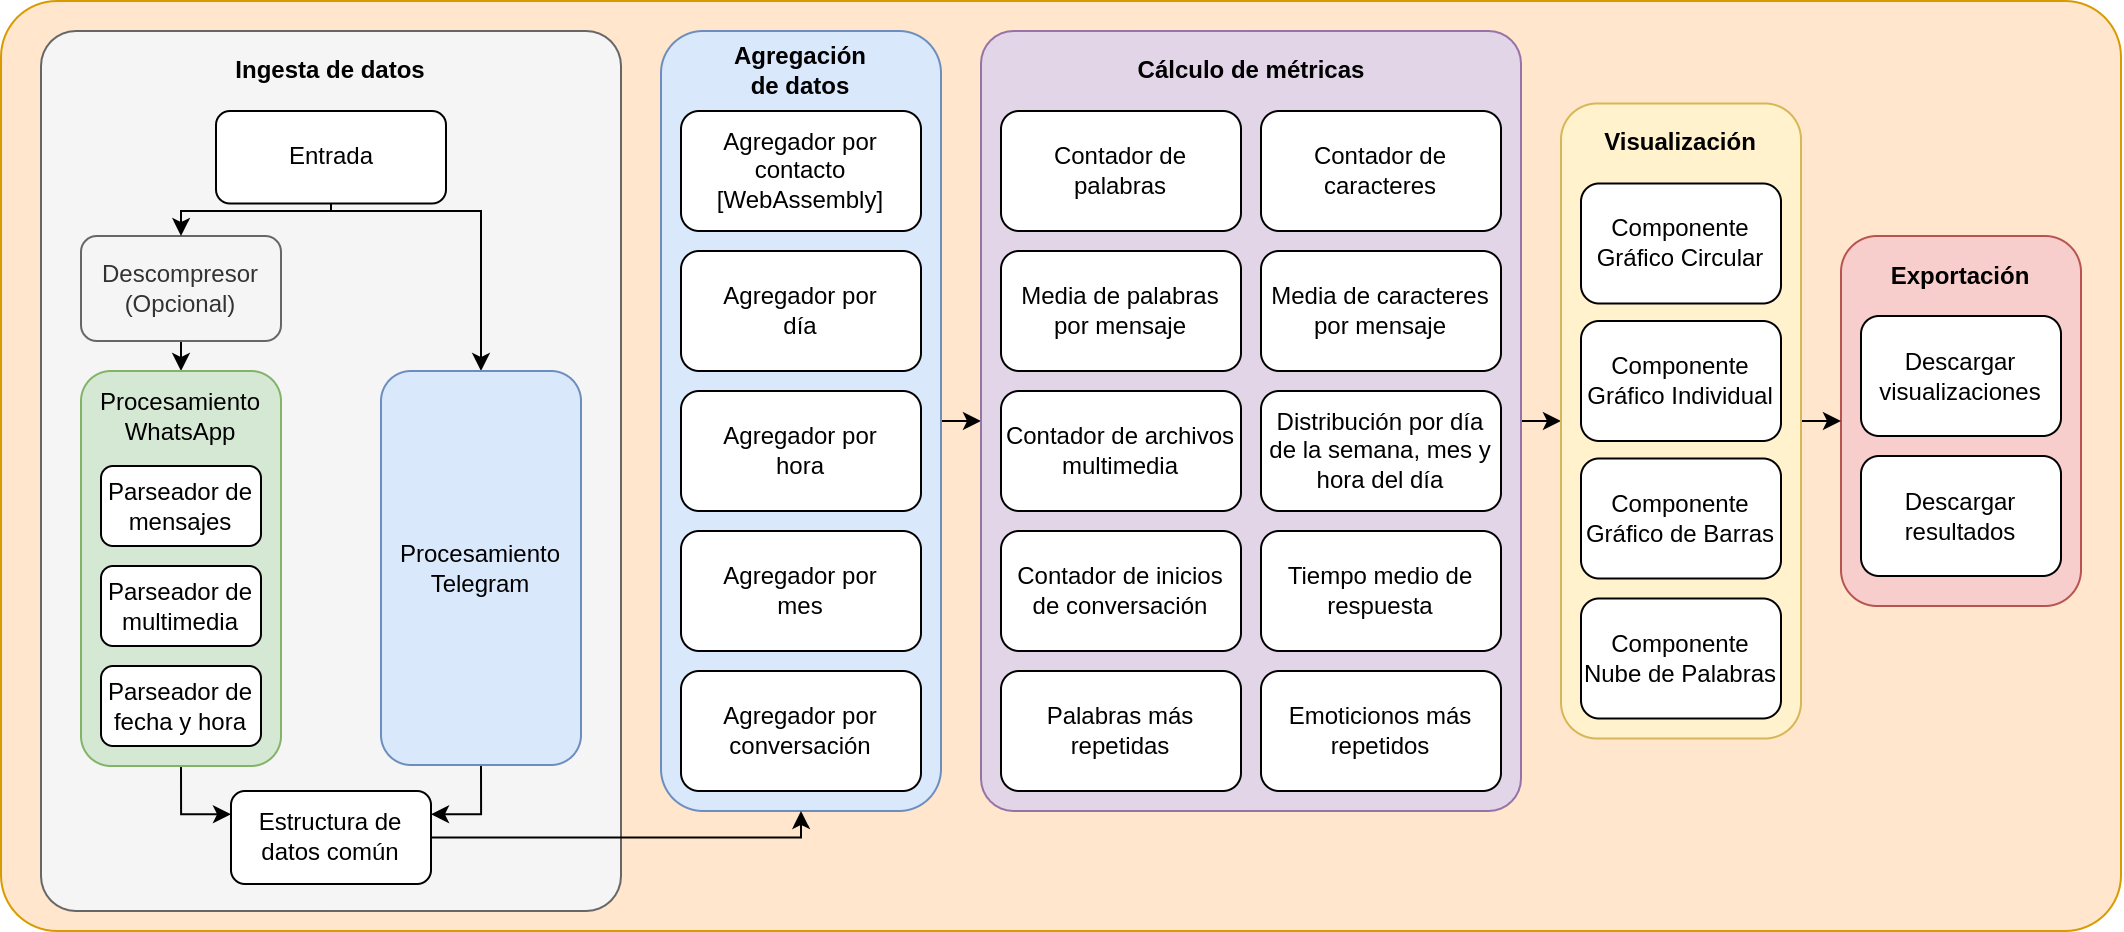
\includegraphics[width=\textwidth]{img/architecture_processing.png}
	\caption{Arquitectura de la aplicación}
	\label{fig:chap4:architecture_processing}
\end{figure}

\subsection{Importador}

El módulo importador se encarga de leer el fichero de entrada. Dicho fichero puede estar en tres formatos diferentes:

\begin{itemize}
	\item \textit{txt} si se trata de un chat exportado de WhatsApp en un dispositivo Android.
	\item \textit{zip} si se trata de un chat exportado de WhatsApp desde un dispositivo iOS.
	\item \textit{\acrshort{json}} si se trata de un chat exportado de Telegram desde la aplicación para escritorio.
\end{itemize}

Aunque Telegram también soporta la exportación de conversaciones en \textit{HTML}, ChatStats no soporta este formato, puesto que está diseñado para la visualización y no para el tratamiento y procesado del mismo.

En caso de exportar el chat con contenido multimedia, ChatStats únicamente espera el fichero de texto plano (ya sea directamente o dentro de un archivo comprimido), puesto que este se encuentran todos los datos necesarios para el análisis del contenido multimedia. Es por ello que todo el contenido multimedia recibido se descarta.

\subsubsection{Entrada}

Este submódulo se encarga de cargar el fichero seleccionado por el usuario, que el navegador ofrece desde una ruta falsa y protegida para que la aplicación no pueda acceder a todos los archivos del dispositivo. En caso de tratarse de un fichero de texto plano, este módulo abre el archivo como una cadena de caracteres. En caso de tratarse de un fichero comprimido, se lo envía al módulo ``Descompresor'' esperando un archivo de texto plano como salida. Por último, en caso de tratarse de cualquier otro tipo de fichero, el módulo alerta al usuario de que el archivo de entrada no es válido.

Este submódulo hace uso de una instancia de \textit{FileReader}; clase que ofrecen los navegadores, permitiendo abrir el fichero como secuencia de caracteres.

\subsubsection{Descompresor (Opcional)}

Este submódulo se encarga de la descompresión de ficheros \textit{zip}, que descomprime bajo petición del módulo anterior. Finalmente, el módulo devuelve un fichero llamado \textit{\_chat.txt}, que, como se ha comentado anteriormente, contiene toda la información necesaria para el análisis (con o sin multimedia).

El descompresor hace uso de la librería \textit{jszip} para la descompresión del fichero. La lógica añadida a esta aplicación nos permite encontrar el fichero de texto plano dentro del fichero comprimido y devolver el mismo al módulo de ``Entrada''.

\subsection{Parseador}

El objetivo de este módulo es estandarizar los datos de entrada con la finalidad de poder utilizar los mismos módulos para cualquier archivo de entrada.

Mientras que Telegram ofrece los datos en formato \acrshort{json}, facilitando así la operabilidad de los mismos; WhatsApp no ofrece una estructura de datos ni consistencia entre distintas versiones de su aplicación.

Se expone a continuación un breve ejemplo del formato utilizado por Telegram:

\begin{lstlisting}[language=JavaScript]
	{
		"name": "group_or_contact_name",
		"type": "private_group_or_private_chat",
		"id": 00000000,
		"messages": [
		...
		{
			"id": 11111,
			"type": "message_service",
			"date": "2019-04-02T20:53:14",
			"date_unixtime": "1554231194",
			"from": "Alice",
			"from_id": "contact_user_id",
			"text": "actual_body_message",
			"text_entities": [
			{
				"type": "plain_link_or_document",
				"text": "actual_body_message"
			}
			]
		},
		{
			"id": 22222,
			"type": "message",
			"date": "2019-05-29T23:46:00",
			"date_unixtime": "1559166360",
			"from": "Bob",
			"from_id": "contact_user_id",
			"reply_to_message_id": 59386,
			"file": "stickers/sticker.webp",
			"thumbnail": "stickers/sticker.webp_thumb.jpg",
			"media_type": "sticker",
			"sticker_emoji": "actual_unicode_emoji",
			"width": 512,
			"height": 341,
			"text": "",
			"text_entities": []
		}, ...
		]
	}
\end{lstlisting}

También se muestra un mensaje en el formato de exportación de WhatsApp en los dispositivos Android:

\begin{lstlisting}
	17/07/2022, 01:28 - Alice: Este es un mensaje de prueba
\end{lstlisting}

Así como un mensaje exportado desde WhatsApp por un dispositivo iOS:

\begin{lstlisting}
	[29/12/22, 0:14:55] Bob: Te escribo desde mi iPhone.
\end{lstlisting}

Podemos observar que, en el caso de WhatsApp, ambos mensajes se componen de la fecha, la hora, el nombre del contacto y el propio cuerpo del mensaje, aunque con distinto formato. Dicha información está disponible también en los mensajes de Telegram.

\subsubsection{Parseador de mensajes}

El objetivo del submódulo es convertir la cadena de caracteres de entrada en mensajes con el siguiente formato \acrshort{json}:

\begin{lstlisting}[language=JavaScript]
	{
		date: new Date("2022-10-17T10:37:00"),
		from: "Juan Pedro",
		text: "IMG-20221020-WA0013.jpg",
		type: "message",
		media_type: "image"
	}
\end{lstlisting}

Hemos decidido esta estructura ya que se trata de toda la información que podemos obtener de mensajes de WhatsApp. Además, es compatible con la estructura ya propuesta por Telegram. Podemos decir entonces que es un máximo común denominador de la información disponible en ambos casos. Serán estos los objetos que se utilizarán más adelante para calcular las estadísticas y las estructuras de datos de visualización.

Es por ello que analizamos ambos casos por separado:

\paragraph{Telegram} En caso de tratar un fichero en formato \acrshort{json}, utiliza la librería \textit{JSON} nativa para \textit{JavaScript}, parseando todo el contenido del módulo ``Importador'' y eliminando los datos del objeto original que no se van a utilizar. Posteriormente, llama al módulo ``Parseador de fecha y hora'' que se describe más adelante.

\paragraph{WhatsApp} En caso de tratar con un fichero de WhatsApp, se llega a la siguiente expresión regular que nos permite separar las partes del mensaje, tanto para Android como para iOS.

\begin{lstlisting}
	/\[*(\d{1,2}\/\d{1,2}\/\d{2,4}),\s(\d{1,2}:\d{2}:*\d*)\]*\s(?:-\s)*(.*?):{1}\s(.*?)(?=\s\[*\d{1,2}\/\d{1,2}\/\d{2,4}|$)/gum
\end{lstlisting}

Los grupos de captura que lo componen se describen en detalle en el \autoref{chap:regex}.


\subsubsection{Parseador de fecha y hora}

Este submódulo tiene como entrada la fecha y la hora. Devuelve un objeto de tipo \textit{Date}, nativo de JavaScript. Esto nos permite realizar operaciones de tiempo con facilidad en otros módulos.

Este submódulo utiliza la librería \textit{momentjs} para parsear los posibles distintos formatos de fecha que utilizan Telegram y WhatsApp en sus cadenas de caracteres. Además, considera el \textit{locale} del cliente, invirtiendo mes y día para el caso \textit{en\_US}.

La salida de este submódulo se utiliza en la clave \textit{``date''} del objeto mensaje del submódulo anterior.

\subsubsection{Parser de archivos multimedia}

Este submódulo se ejecuta únicamente para chats exportados por WhatsApp. El objetivo de este submódulo es escribir el tipo de contenido en la clave \textit{``media\_type''} del objeto mensaje expuesto anteriormente.

Existen dos opciones para exportar un chat: con contenido multimedia o sin él.

\paragraph{Para contenido multimedia}\mbox{}\\

En el fichero de texto plano con contenido multimedia, observaremos que el cuerpo incluye el nombre del fichero que se ha exportado con la extensión del formato del mismo. Por ello, categorizamos como \textit{voice\_message}, \textit{video\_file}, \textit{sticker} o \textit{image} en función a la extensión; \textit{.opus}, \textit{.mp4}, \textit{.webp} o \textit{.jpg}, respectivamente. Usamos estos valores puesto que son los que Telegram utiliza para su formato de mensajes.

Se indican a continuación mensajes de ejemplo para cada tipo de archivo adjunto, únicamente para Android:

\begin{lstlisting}
	17/10/2022, 21:11 - Juan Pedro: PTT-20221017-WA0078.opus (file attached)
	20/10/2022, 10:37 - Juan Pedro: IMG-20221020-WA0013.jpg (file attached)
	14/11/2022, 18:58 - Juan Pedro: VID-20221114-WA0039.mp4 (file attached)
	24/11/2022, 19:13 - Jaime Conde: STK-20220717-WA0090.webp (file attached)
\end{lstlisting}

\paragraph{Sin contenido multimedia}\mbox{}\\

Para el segundo caso, cada vez que un mensaje sea contenido multimedia, aparecerá \textit{\textless Media omitted \textgreater} (multimedia omitido). Estos pueden ser fotos, vídeos, música, notas de voz o documentos. Se definirán como \textit{undefined} o indefinidos, ignorándose en las visualizaciones y módulos posteriores.

\begin{lstlisting}
	17/07/2022, 01:33 - Juan Pedro: <Media omitted>
\end{lstlisting}

\subsection{Agregador}

Los mensajes se encuentran segregados en una lista, por lo que a continuación, el módulo de agregador se encargará de agregar los mensajes en diferentes grupos. En el código los hemos llamado polarizadores. Se describen los distintos submódulos a continuación:

\subsubsection{Agregador por contacto}

\textit{ChatStats} se encarga de calcular las estadísticas de cada contacto para visualizarlas y mostrarlas en comparación con el resto de contactos. Hablamos de numerosos contactos, puesto que es compatible con chats individuales y grupales.

El resultado de este submódulo será un objeto \acrshort{json} con una clave por cada contacto (su nombre), que contendrá un array de los mensajes enviados por este. Se indica un ejemplo:

\begin{lstlisting}[language=JavaScript]
	{
		"Jaime": [...messagesByJaime],
		"Juan Pedro": [...messagesByJuanPedro],
		...
	}
\end{lstlisting}

donde los array de mensajes contienen objetos definidos en el \textit{Parser de mensajes}.

\subsubsection{Agregador por día}

Este agregador toma como entrada la salida del submódulo anterior: los mensajes agregados por contacto. Con ello se procede a agregarlos, además, por día de la semana: de lunes a domingo. Se usará el nombre del día de la semana como clave anidada.

El resultado son objetos con la siguiente estructura:

\begin{lstlisting}[language=JavaScript]
	{
		"Jaime": {
			"monday": [...messagesByJaimeOnMonday],
			"tuesday": [...messagesByJaimeOnTuesday],
			...,
			"sunday": [...messagesByJaimeOnSunday]
			},
		"Juan Pedro": {
			"monday": [...messagesByJuanPedroOnMonday],
			"tuesday": [...messagesByJuanPedroOnTuesday],
			...,
			"sunday": [...messagesByJuanPedroOnSunday]
		},
		...
	}
\end{lstlisting}

El objetivo de esta estructura de datos es visualizar la distribución de los mensajes a lo largo de la semana, en media.

\begin{comment}
	Se deja para futuras líneas un gráfico en el que se pueda elegir el año a analizar, o un scroll vertical por años.
\end{comment}

\subsubsection{Agregador por hora}

Este agregador toma también como entrada los mensajes agregados por contacto. Con ello se procede a agregarlos, además, por hora del día, usando la hora en formato 24 horas como clave anidada de agregación: de 00 a 23 horas.

El resultado son objetos con la siguiente estructura:

\begin{lstlisting}[language=JavaScript]
	{
		"Jaime": {
			"00": [...messagesByJaimeAt00],
			"01": [...messagesByJaimeAt01],
			...,
			"23": [...messagesByJaimeAt23]
		},
		"Juan Pedro": {
			"00": [...messagesByJuanPedroAt00],
			"01": [...messagesByJuanPedroAt01],
			...,
			"23": [...messagesByJuanPedroAt23]
		},
		...
	}
\end{lstlisting}

El objetivo de esta estructura de datos es visualizar la distribución de los mensajes a lo largo del día, en media.

\subsubsection{Agregador por mes}

Este agregador toma también como entrada los mensajes agregados por contacto. Con ello se procede a agregarlos, además, por MM/YYYY, por lo que deja de tratarse de un agregador acotado: pueden haber tantas claves anidadas como meses se haya hablado.

El resultado son objetos con la siguiente estructura:

\begin{lstlisting}[language=JavaScript]
	{
		"Jaime": {
			"10/2022": [...messagesByJaimeOnOctober2022],
			"11/2022": [...messagesByJaimeOnNovember2022],
			...
		},
		"Juan Pedro": {
			"10/2022": [...messagesByJuanPedroOnOctober2022],
			"11/2022": [...messagesByJuanPedroOnNovember2022],
			...
		},
		...
	}
\end{lstlisting}

El objetivo de esta estructura de datos es visualizar la distribución de los mensajes a lo largo del tiempo, con una agregación mensual.

\subsubsection{Agregador por conversación}

Este submódulo analiza las diferencias de tiempos entre los mensajes, categorizándolos como inicio de conversación si son el primer mensaje en las últimas 5 horas, o como respuesta si se trata de un intervalo de tiempo menor. Esto nos permitirá calcular cuántas conversaciones ha iniciado cada contacto, así como el tiempo de respuesta medio de cada uno; módulos que se verán más adelante.

Aunque un sesgo temporal no es una solución perfecta, acierta gran parte de las veces sin necesitar gran capacidad de cómputo.

\subsection{Visualizador}

Este módulo prepara los datos para ser representados por la librería de visualización elegida: \textit{ChartJS}.  Esta librería ha sido elegida por su alta actividad de contribuciones al proyecto, que es libre y cuenta con 12 mil estrellas en GitHub. Además, permite alta extensibilidad mediante plugins, de los que hacemos uso, por ejemplo, para mostrar las etiquetas de los datos.

Cada módulo aquí desarrollado realiza el cálculo de una métrica, cuyo resultado pasa por una función que adapta el contenido a la estructura solicitada por \textit{ChartJS}. \textit{ChartJS} nos permite un único formato de entrada para los datos, permitiéndonos elegir el tipo de gráfico de forma independiente a dichos datos. Esta arquitectura nos permite añadir más módulos posteriormente; realizando el cálculo de la métrica a mostrar y pasándolo por la función que estandariza los datos para \textit{ChartJS}.

Todos los submódulos que utilizan \textit{ChartJS} adaptan el tamaño del gráfico al número de contactos que hay en el grupo de forma \textit{responsive}. También permiten la interacción con el mismo, pudiendo eliminar contactos de la representación haciendo click sobre el nombre de los mismos en la leyenda.

Además, también se procesan datos para otras librerías de visualización, como \textit{react-wordcloud}, para las nubes de palabras o \textit{word clouds} y nubes de emoticonos.

\subsubsection{Contador de mensajes}

Este submódulo cuenta el número de mensajes enviado por cada contacto. Para chats grupales, usa la librería \textit{ChartJS}, mientras que para chat individuales, únicamente se exponen los números de ambas partes directamente.

\begin{figure}[H]
	\centering
	\subfloat[\centering Chat individual]{{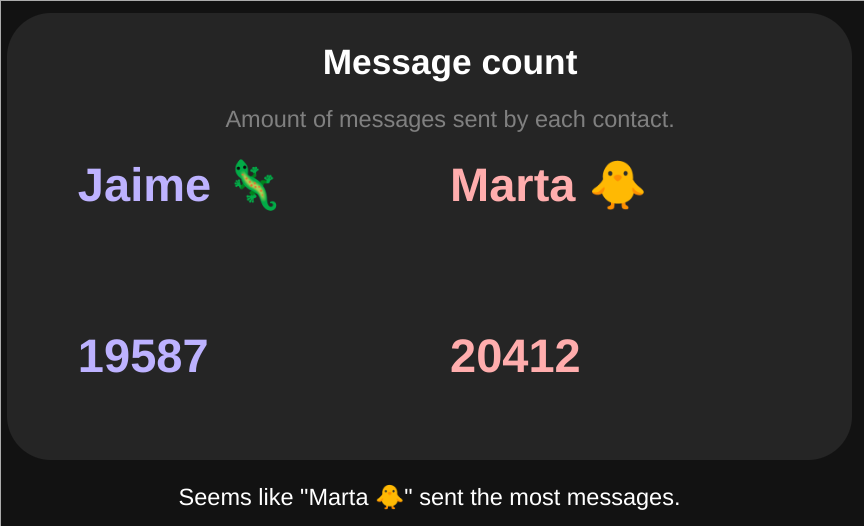
\includegraphics[width=6cm]{img/message_count_individual.png} }}
	\qquad
	\subfloat[\centering Chat grupal]{{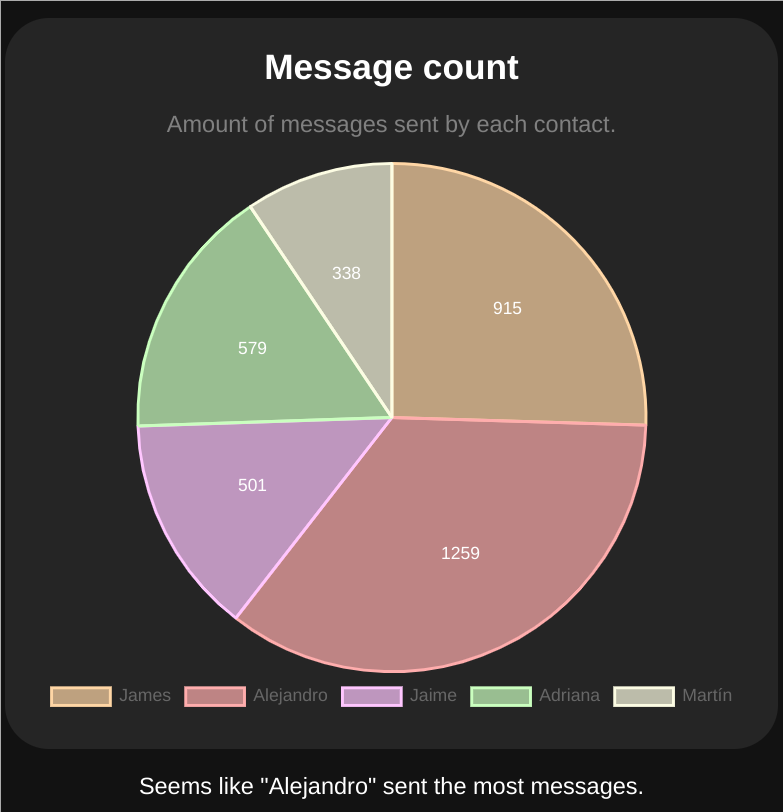
\includegraphics[width=6cm]{img/message_count.png} }}
	\caption{Contador de mensajes}
	\label{fig:chap4:message_count}
\end{figure}

Se ha optado por calcular esta métrica puesto que puede ayudar a observar diferencias drásticas en la cantidad de texto que aporta cada contacto.

\subsubsection{Contador de palabras}

Este submódulo cuenta las palabras que hay en los mensajes de cada contacto y calcula la suma total de las mismas, obteniendo el número de palabras totales enviadas por cada contacto. Para chats grupales, usa la librería \textit{ChartJS}, mientras que para chat individuales, únicamente se exponen los números de ambas partes directamente.

\begin{figure}[H]
	\centering
	\subfloat[\centering Chat individual]{{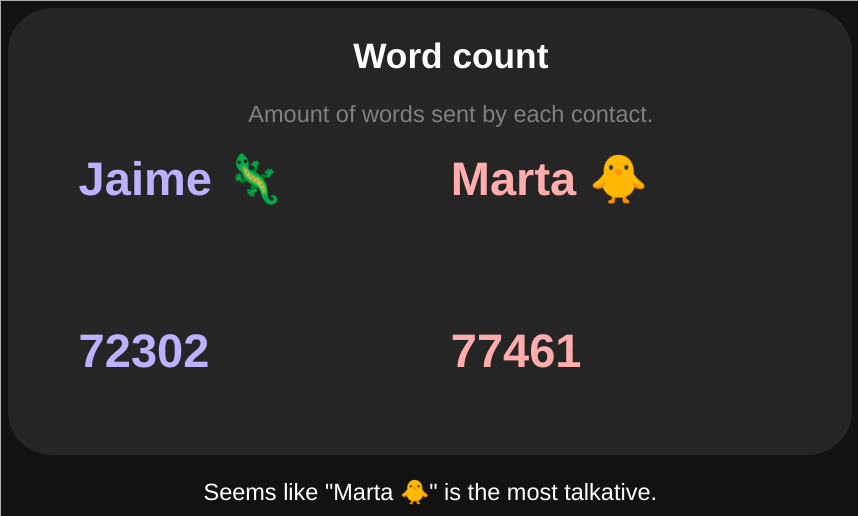
\includegraphics[width=6cm]{img/word_count_individual.png} }}
	\qquad
	\subfloat[\centering Chat grupal]{{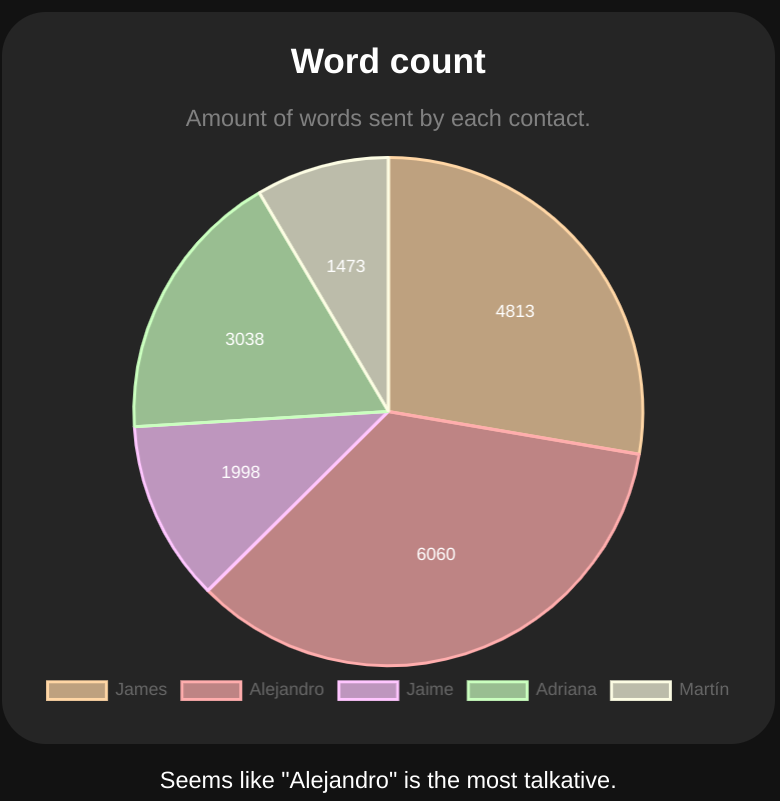
\includegraphics[width=6cm]{img/word_count.png} }}
	\caption{Contador de palabras}
	\label{fig:chap4:word_count}
\end{figure}

\subsubsection{Contador de caracteres}

Este submódulo cuenta los caracteres que hay en los mensajes de cada contacto y calcula la suma total de los mismos, obteniendo el número de caracteres totales enviados por cada contacto. Aunque suele indicar resultados similares al módulo anterior, en algunas ocasiones es distinto, por lo que se ha decidido incluir también.

\begin{figure}[H]
	\centering
	\subfloat[\centering Chat individual]{{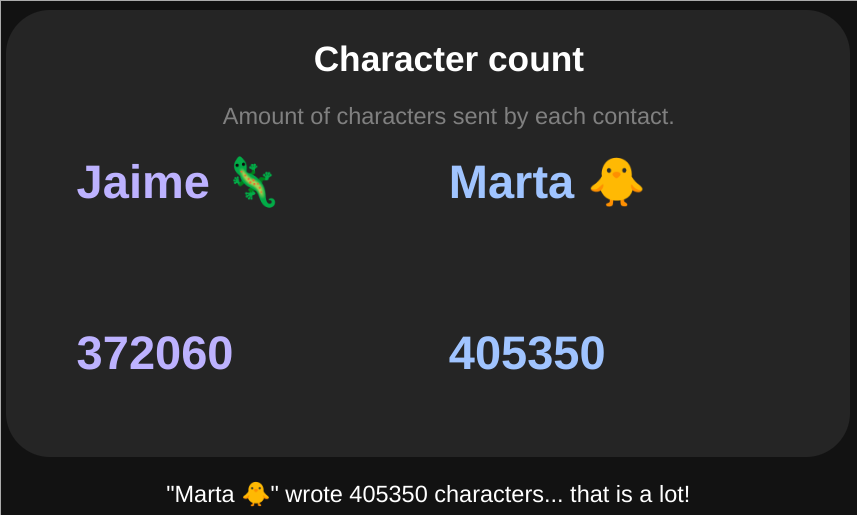
\includegraphics[width=6cm]{img/char_count_individual.png} }}
	\qquad
	\subfloat[\centering Chat grupal]{{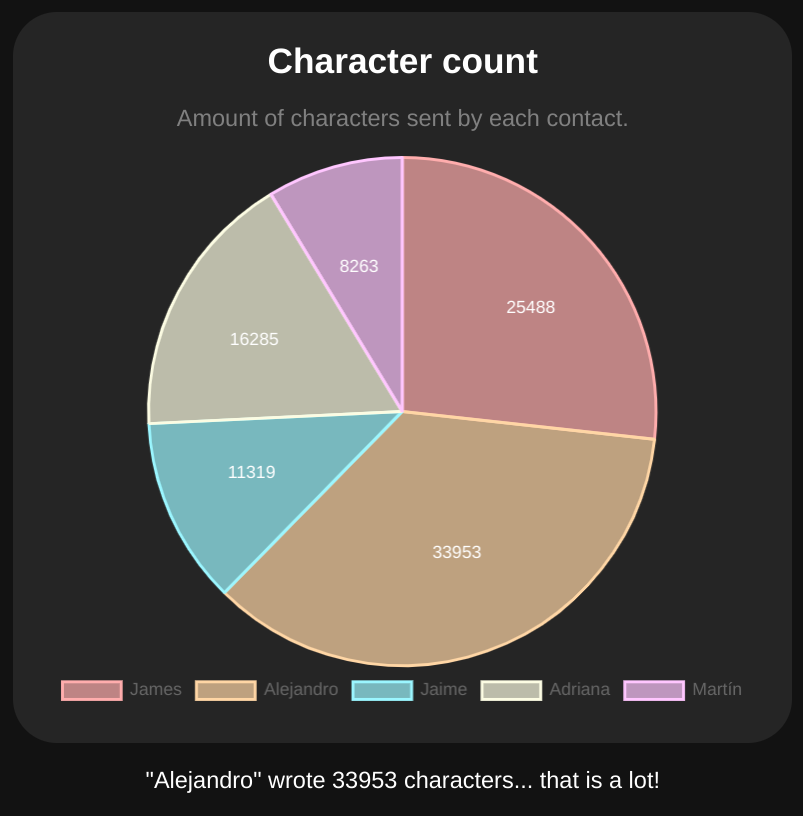
\includegraphics[width=6cm]{img/char_count.png} }}
	\caption{Contador de caracteres}
	\label{fig:chap4:char_count}
\end{figure}

De nuevo, para chats grupales, usa la librería \textit{ChartJS}, mientras que para chat individuales, únicamente se exponen los números de ambas partes directamente.

\subsubsection{Media de palabras por mensaje}

Este submódulo calcula y muestra el número medio de palabras por mensaje para cada contacto. Esta métrica puede ayudar, junto con el número de mensajes totales, a saber si un contacto tiende a mandar más mensajes con menor número de palabras, o menos mensajes con más palabras.

\begin{figure}[H]
	\centering
	\subfloat[\centering Chat individual]{{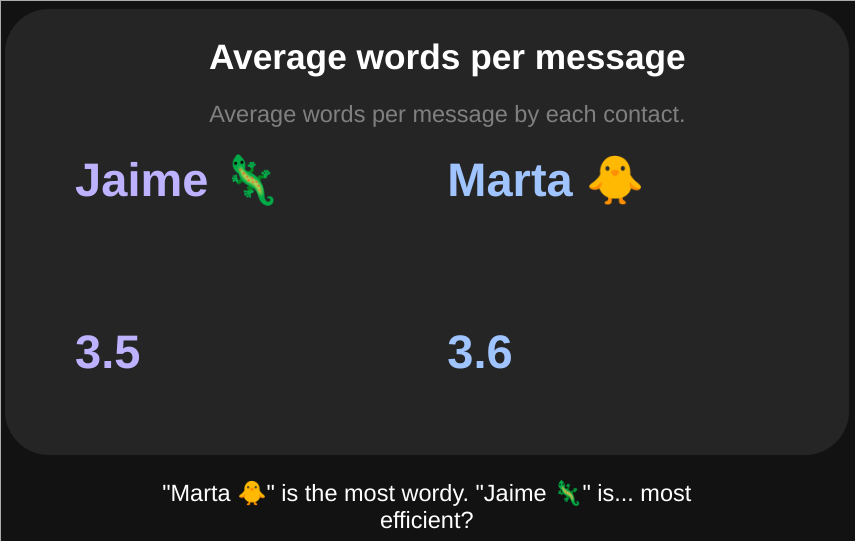
\includegraphics[width=6cm]{img/word_avg_individual.png} }}
	\qquad
	\subfloat[\centering Chat grupal]{{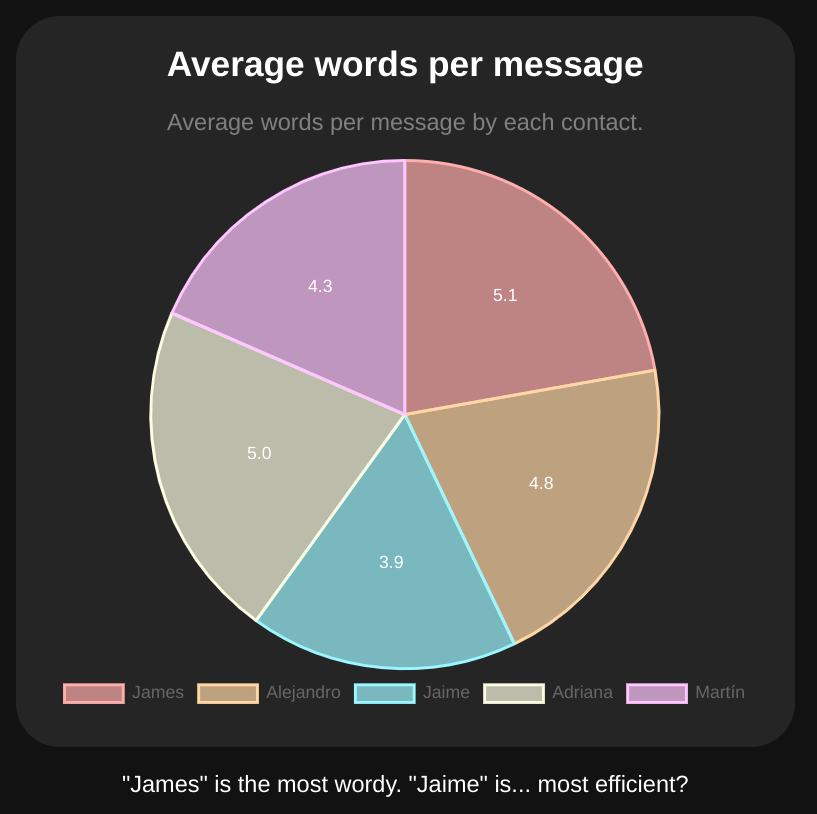
\includegraphics[width=6cm]{img/word_avg.png} }}
	\caption{Media de palabras por mensaje}
	\label{fig:chap4:word_avg}
\end{figure}

\subsubsection{Media de caracteres por mensaje}

Este submódulo calcula y muestra el número medio de caracteres por mensaje para cada contacto. Aunque suele indicar resultados similares al módulo anterior, en algunas ocasiones puede resaltar personas que tienden a usar palabras más largas.

\begin{figure}[H]
	\centering
	\subfloat[\centering Chat individual]{{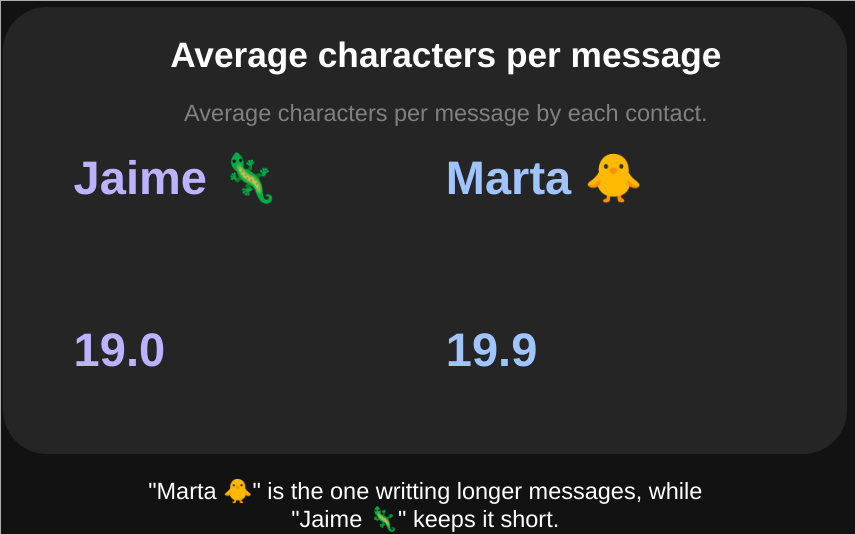
\includegraphics[width=6cm]{img/char_avg_individual.png} }}
	\qquad
	\subfloat[\centering Chat grupal]{{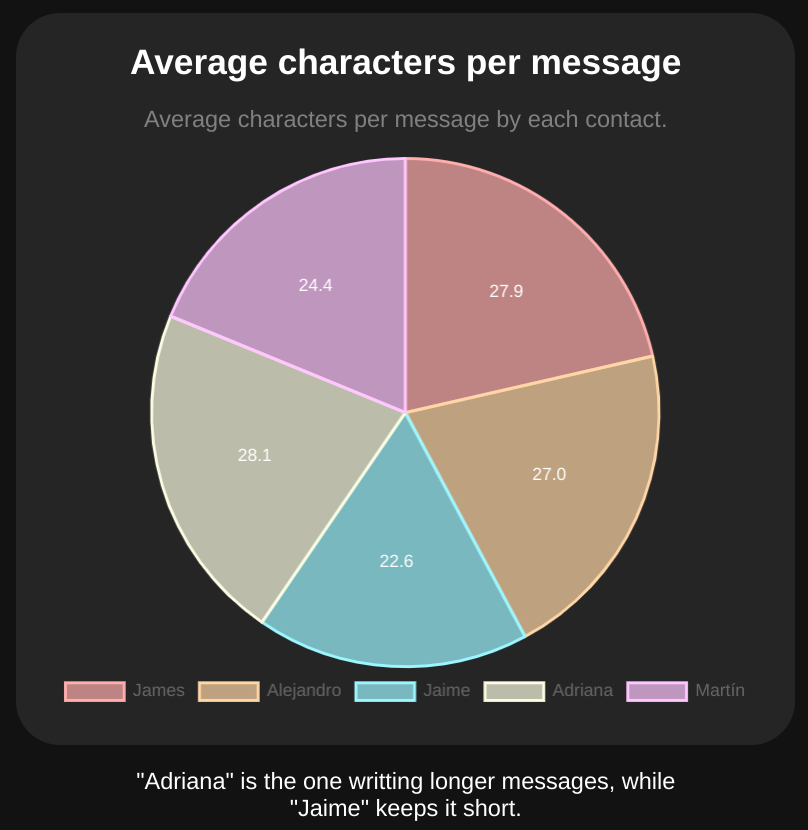
\includegraphics[width=6cm]{img/char_avg.png} }}
	\caption{Media de caracteres por mensaje}
	\label{fig:chap4:char_avg}
\end{figure}

\subsubsection{Número de conversaciones iniciadas}

Este submódulo calcula el número de veces que cada contacto ha iniciado la conversación, con los criterios y datos obtenidos del módulo ``Agregador por conversación''. Se ha decidido calcular esta métrica puesto que es una buena forma de medir la iniciativa de una persona, así como su interés en el grupo o persona individual.

\begin{figure}[H]
	\centering
	\subfloat[\centering Chat individual]{{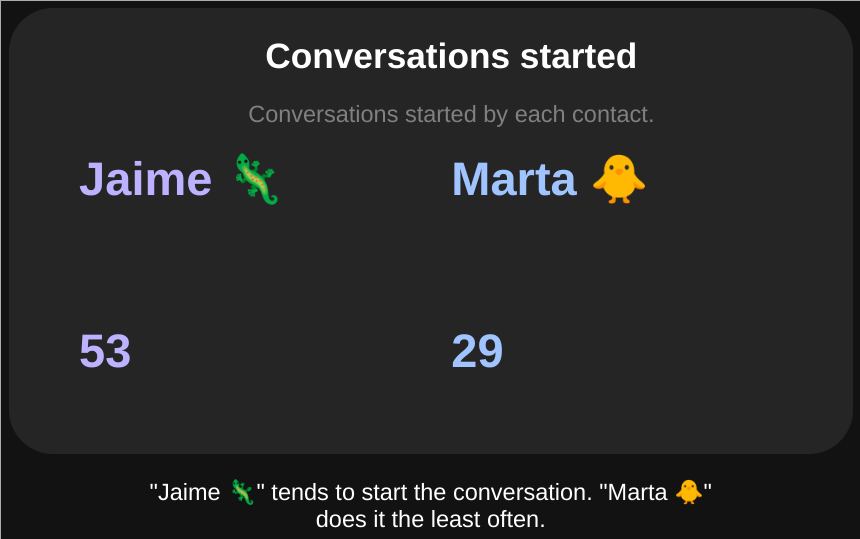
\includegraphics[width=6cm]{img/conversations_started_individual.png} }}
	\qquad
	\subfloat[\centering Chat grupal]{{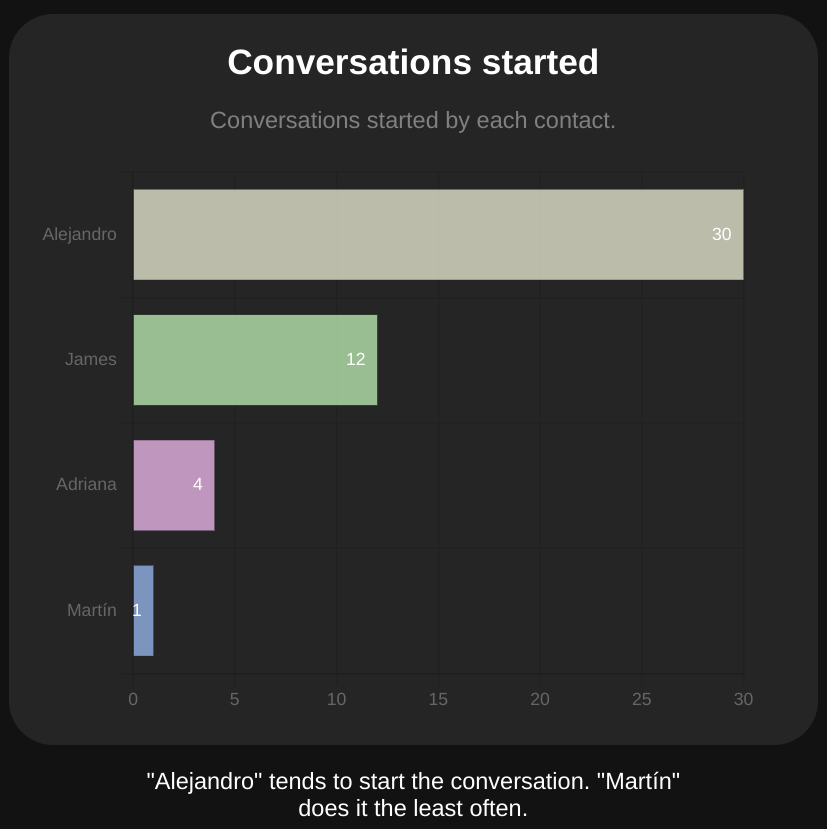
\includegraphics[width=6cm]{img/conversations_started.png} }}
	\caption{Conversaciones iniciadas por cada contacto}
	\label{fig:chap4:conversations_started}
\end{figure}

En este ejemplo, podemos ver cómo Alejandro, el presidente de la asociación, suele tomar la iniciativa y comenzar las conversaciones.


\subsubsection{Velocidad media de respuesta}

Este submódulo calcula la velocidad media de respuesta de cada contacto, con los criterios y datos obtenidos del módulo ``Agregador por conversación''. Se ha decidido calcular esta métrica puesto que es una buena forma de medir la atención a la aplicación de mensajería instantánea, así como la importancia que le da al grupo.

\begin{figure}[H]
	\centering
	\subfloat[\centering Chat individual]{{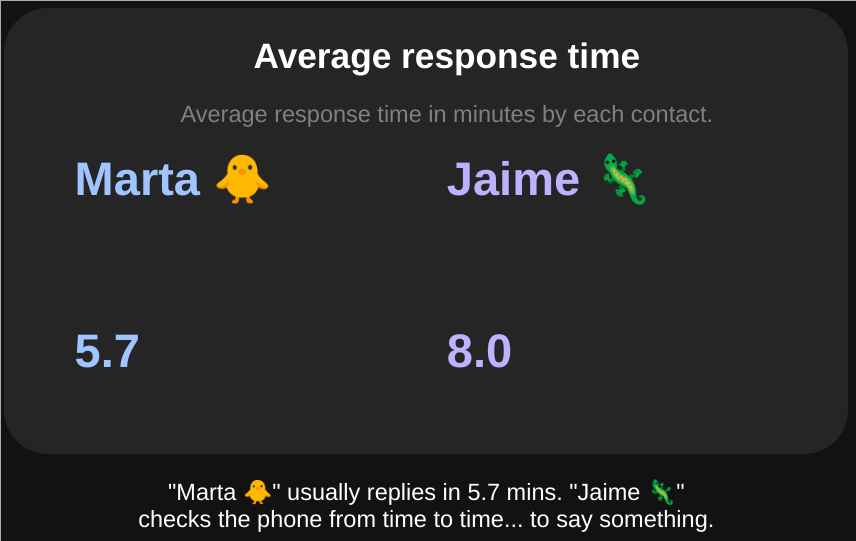
\includegraphics[width=6cm]{img/avg_response_time_individual.png} }}
	\qquad
	\subfloat[\centering Chat grupal]{{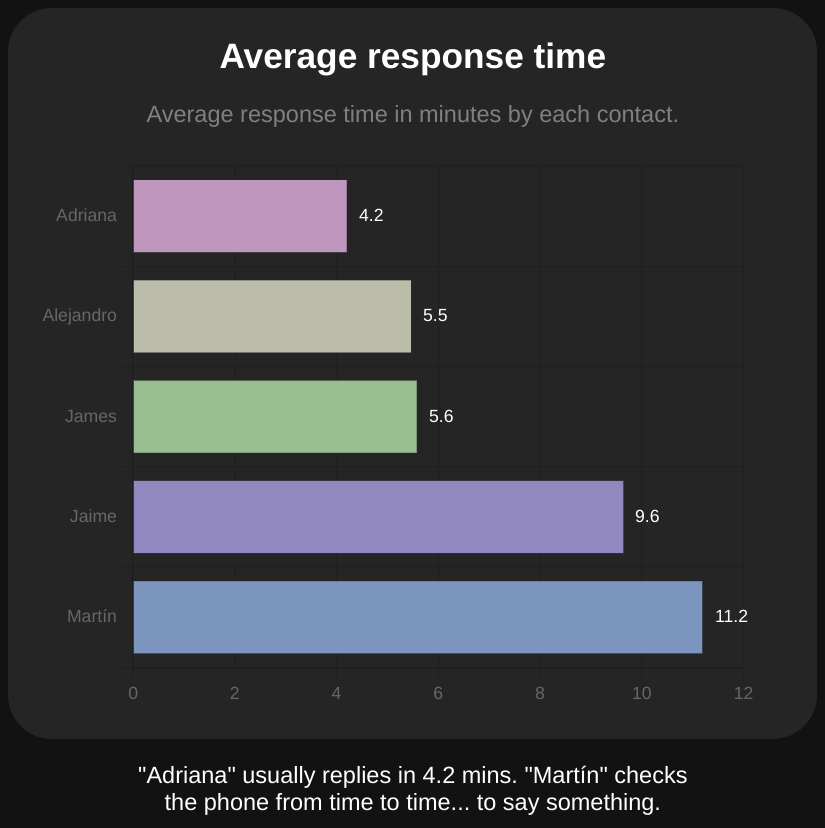
\includegraphics[width=6cm]{img/avg_response_time.png} }}
	\caption{Tiempo medio de respuesta}
	\label{fig:chap4:avg_response_time}
\end{figure}

Añadiendo esta figura a la anterior, podemos ver cómo Martín inicia pocas conversaciones y, además, suele tardar bastante en responder. Esto puede sugerir que está menos involucrado en el grupo.


\subsubsection{Contador de multimedia}

En caso de que existan objetos \acrshort{json} con el campo ``\textit{media\_type}'' distinto de \textit{undefined}, este submódulo cuenta cuántos archivos multimedia de cada tipo ha mandado cada contacto.


\begin{figure}[h]
	\centering
	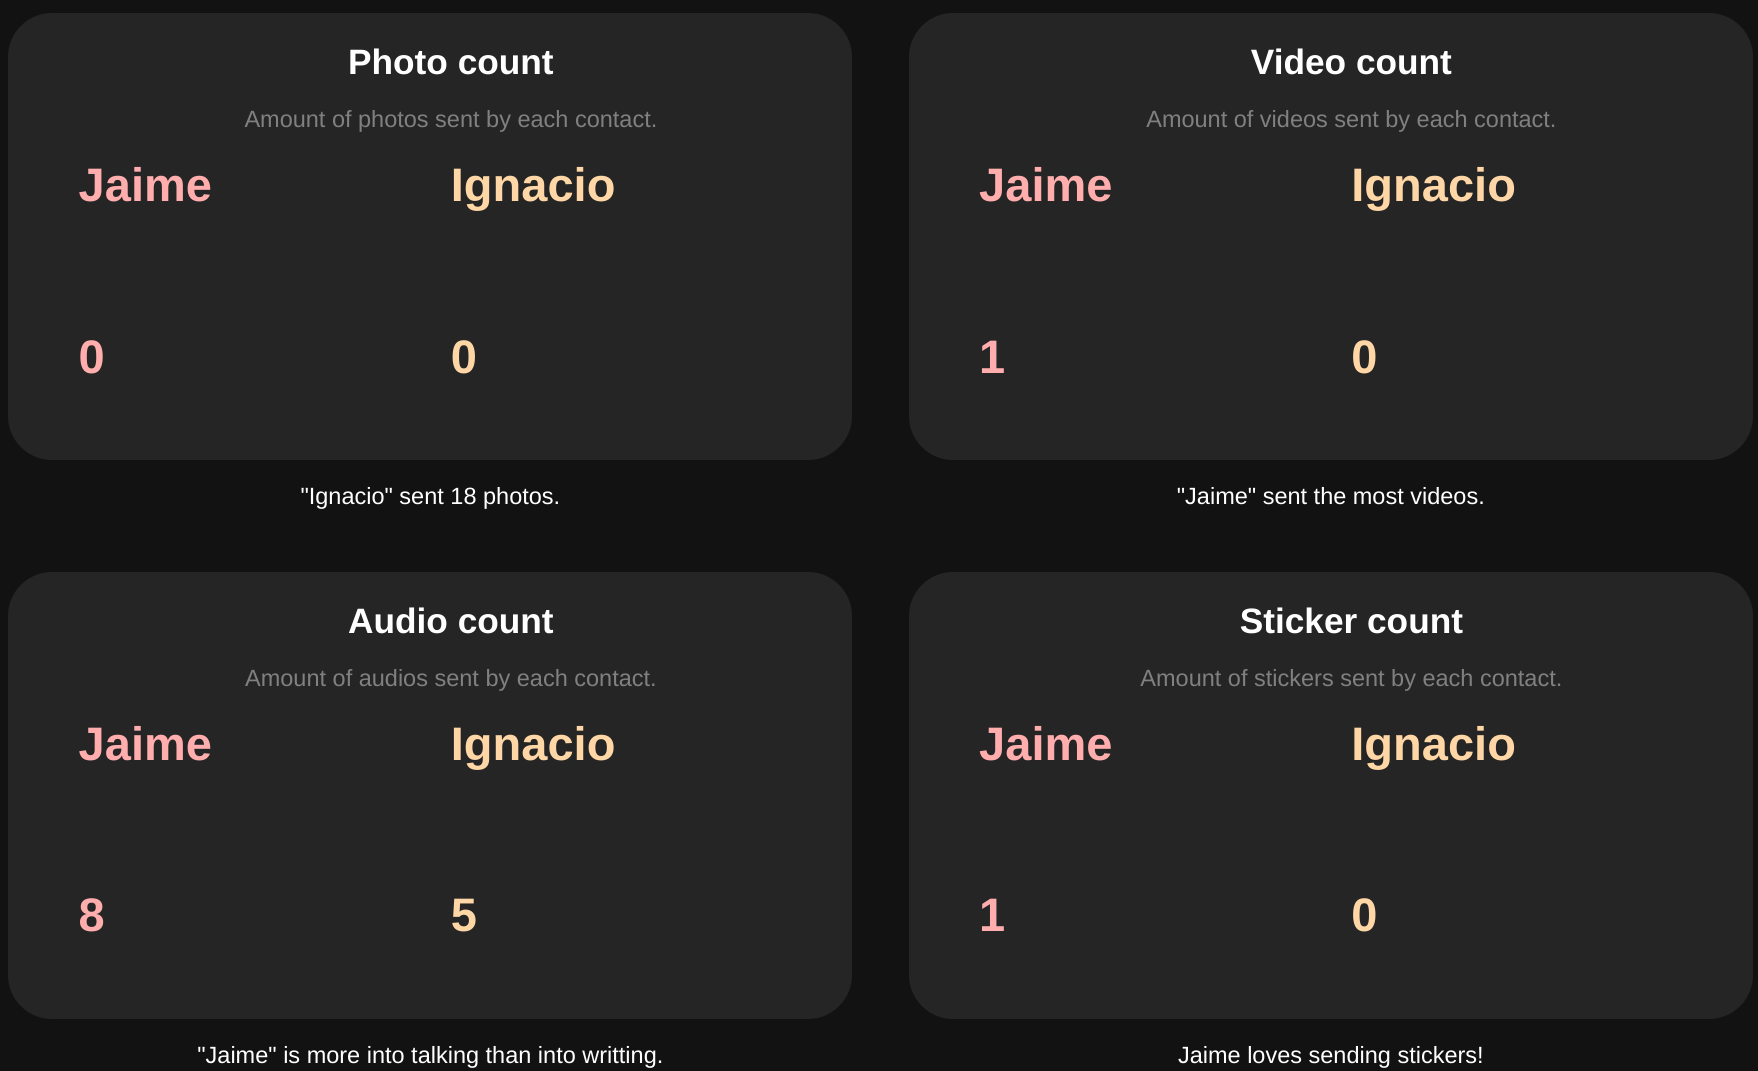
\includegraphics[width=0.8\textwidth]{img/media_count_individual.png}
	\caption{Contador de multimedia para chats individuales}
	\label{fig:chap4:media_count_individual}
\end{figure}


\begin{figure}[h]
	\centering
	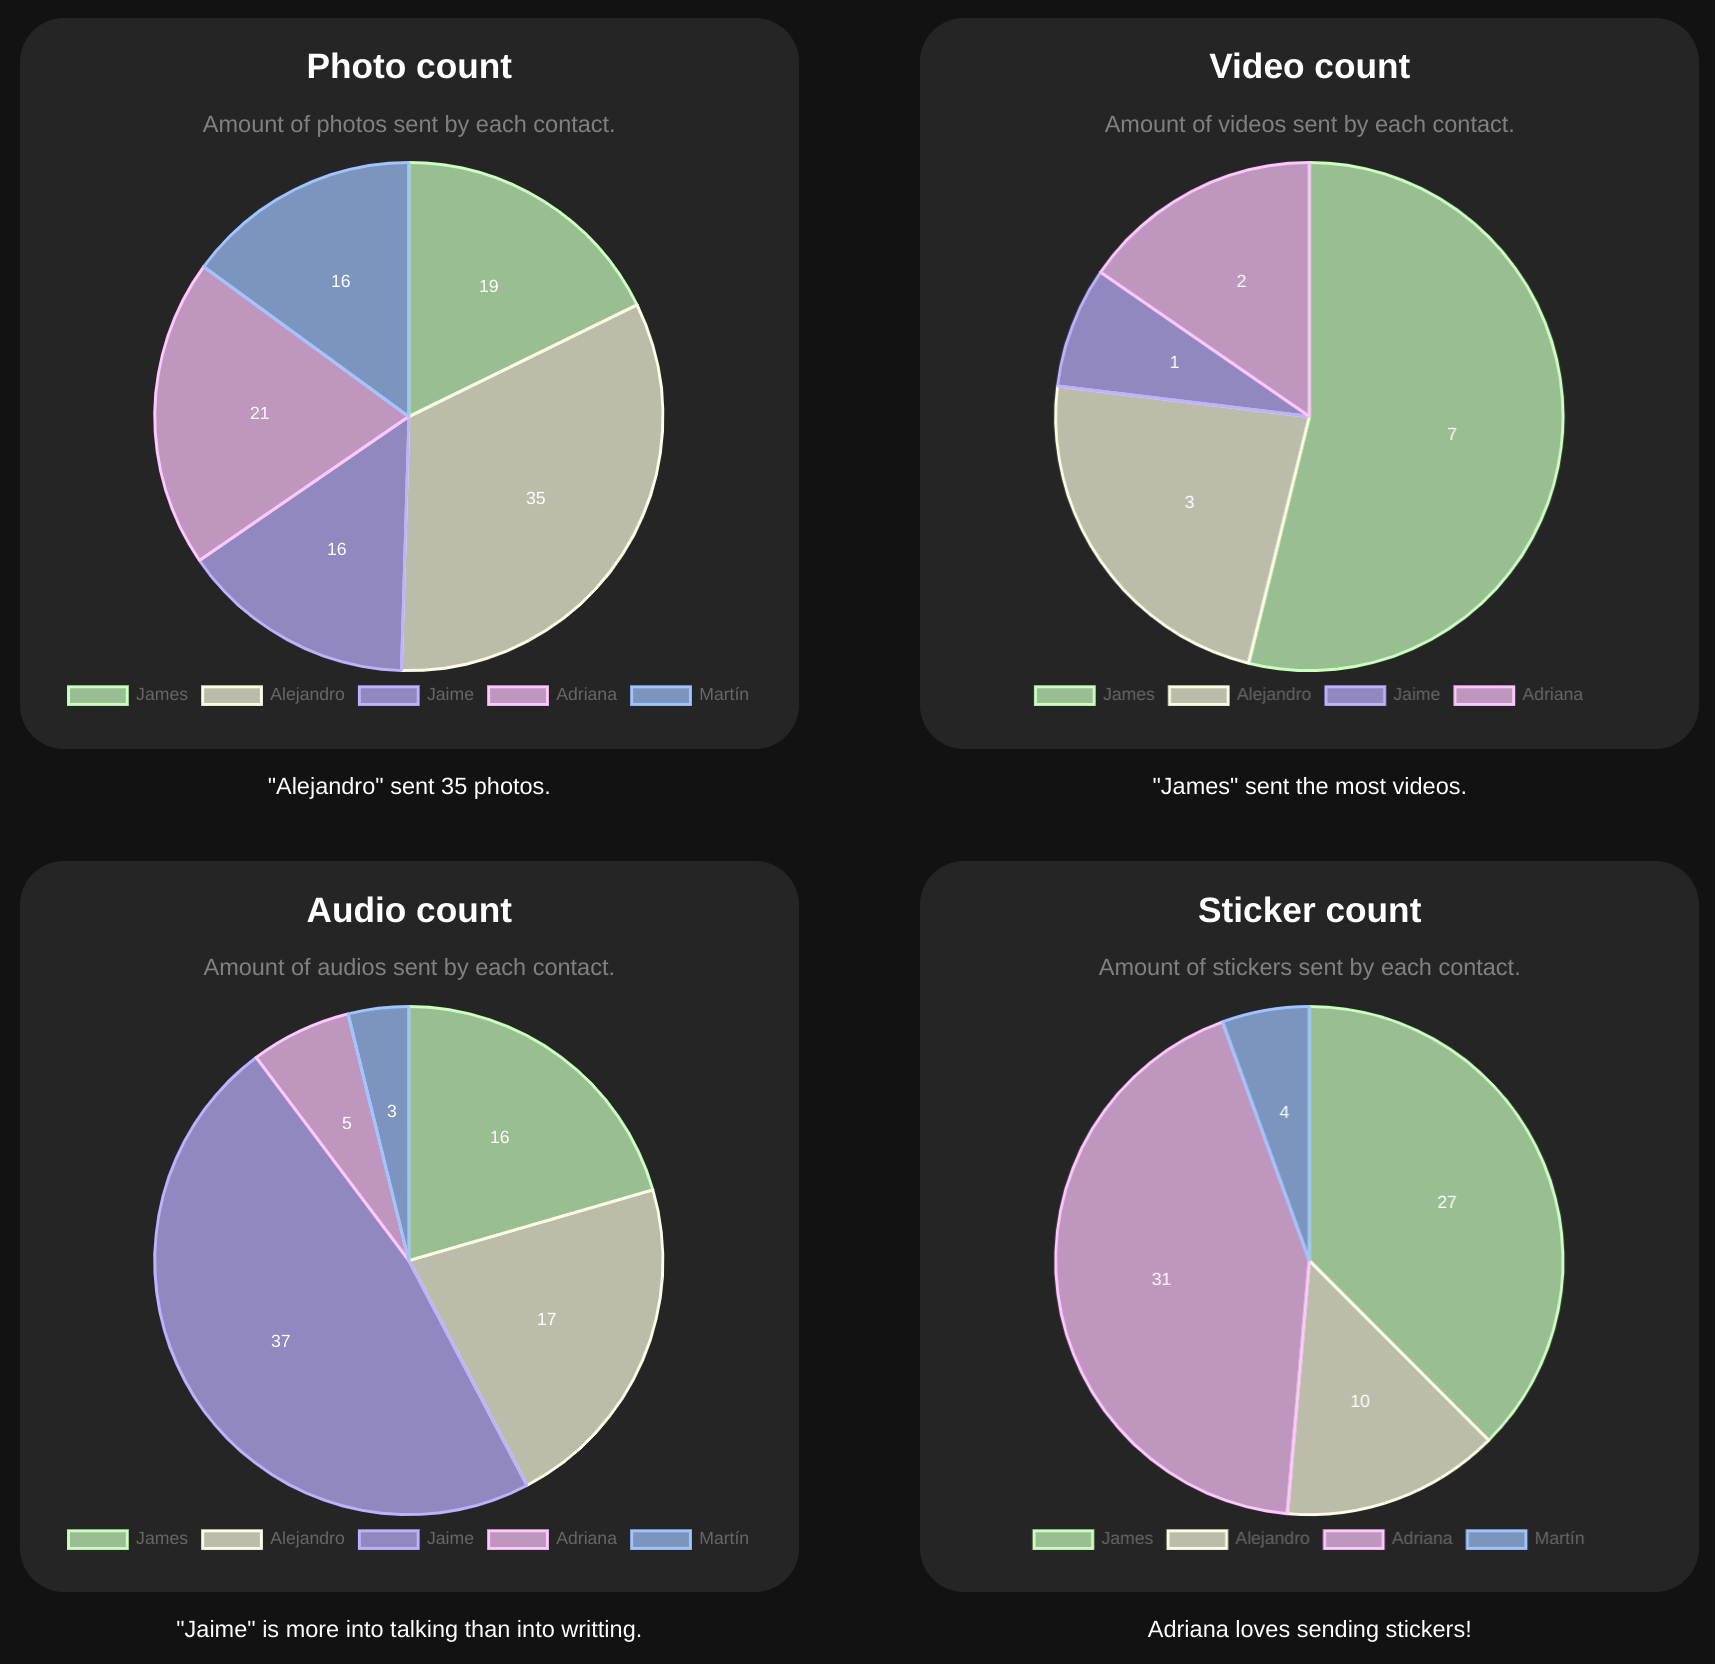
\includegraphics[width=0.7\textwidth]{img/media_count.png}
	\caption{Contador de multimedia para chats grupales}
	\label{fig:chap4:media_count}
\end{figure}

\subsubsection{Generador de estructuras de datos por día, hora y mes}

Para el gráfico de barras con el número de mensajes en el tiempo, \textit{ChartJS} necesita una estructura de datos para mensajes por día, siendo los días la variable independiente y el número de mensajes la variable dependiente.

\begin{figure}[H]
	\centering
	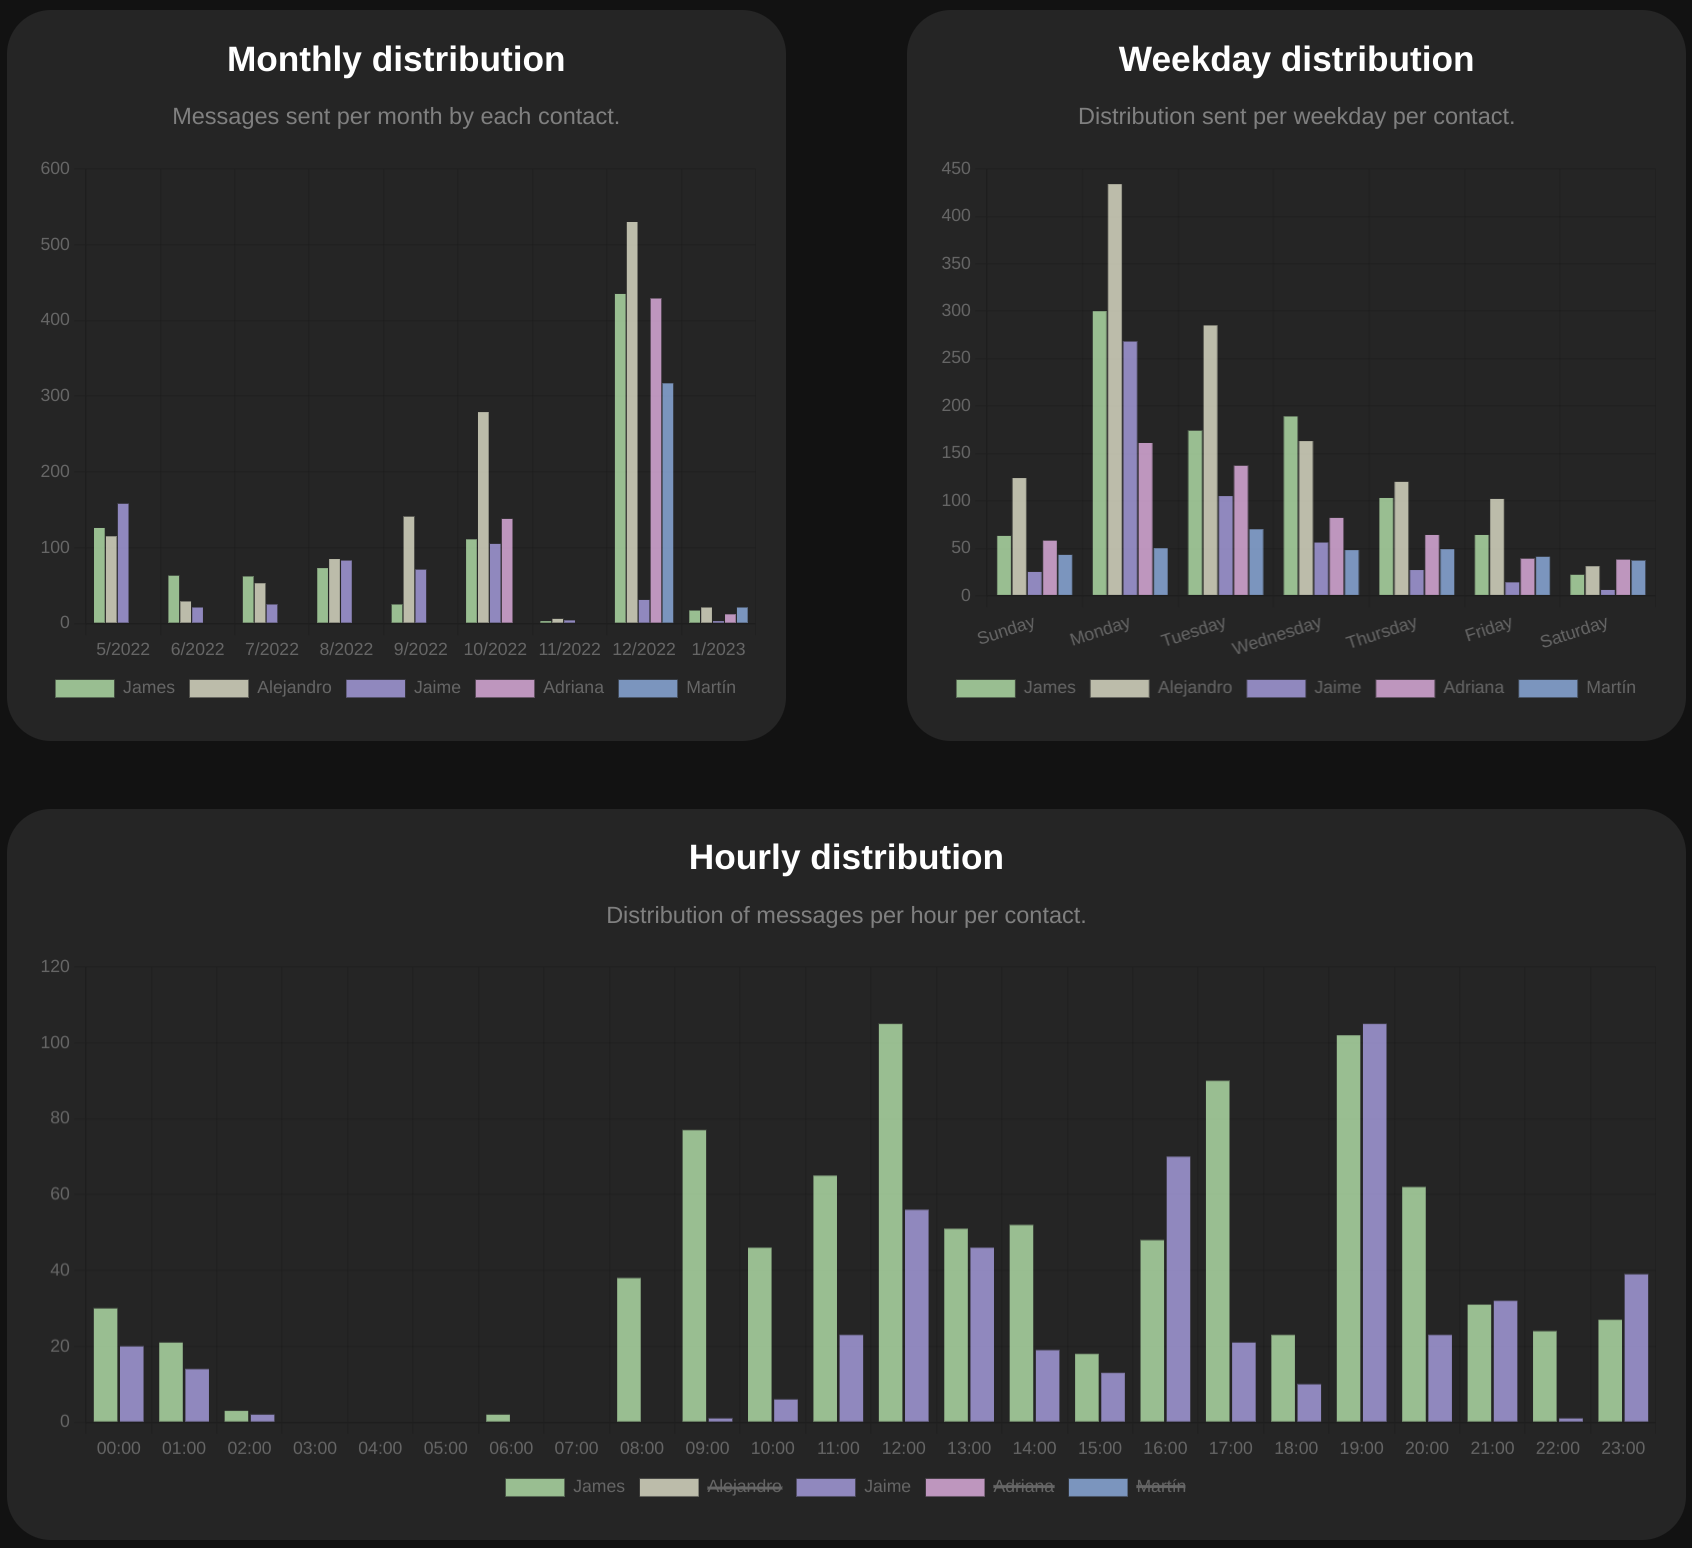
\includegraphics[width=0.7\textwidth]{img/time_distributions.png}
	\caption{Distribuciones en el tiempo}
	\label{fig:chap4:time_distributions}
\end{figure}

Se elige calcular y mostrar estas distribuciones puesto que ayudan a observar la evolución en el tiempo de la cantidad de mensajes intercambiados, así como los días de la semana más activos. Por ejemplo una pareja que pasa los fines de semana juntos tendrá menos mensajes los fines de semana. Por último, la distribución en las 24 horas del día ayuda a analizar las horas pico de conversación, así como las horas de final e inicio del día para cada contacto.

Para la distribución por horas en el día, se ha planteado también usar un gráfico de araña o radar, pero dicha opción se descartó al observar el solapamiento que tenía lugar con varios contactos.

En la figura podemos observar cómo el contacto Jaime comienza a mandar mensajes a las 9 de la mañana, mientras que James suele comenzar 2 horas antes: a las 7 de la mañana. Esto sugiere que James comienza antes el día, o Jaime no utiliza el móvil hasta las 9 de la mañana.

\subsubsection{Contador de palabras más repetidas}

Este submódulo procesa todas las palabras de los mensajes, elimina las palabras más comunes del español y el inglés, así como otros mensajes que WhatsApp añade, como \textit{Media ommited} o \textit{This message has been deleted}.

Las listas de palabras más comunes del español e inglés se han recopilado de distintas fuentes, combinado y eliminado repeticiones.

A la salida de este módulo, se muestra un diccionario con las palabras más repetidas y el número de veces que aparece cada una; información de la que hará uso la librería \textit{react-wordcloud}. Esta información resulta útil para resaltar los temas principales tratados en el chat.

Puede observarse en la \autoref{fig:chap4:word_emoji_cloud}

\subsubsection{Contador de emoticonos más usados}

Este módulo aplica una expresión regular unicode a todos los mensajes, seleccionando los emoticonos y contando el número de veces que aparecen. Posteriormente otra nube de palabras hace uso de esta información por medio de la librería \textit{react-wordcloud}.

\begin{figure}[H]
	\centering
	\subfloat[\centering Nube de palabras]{{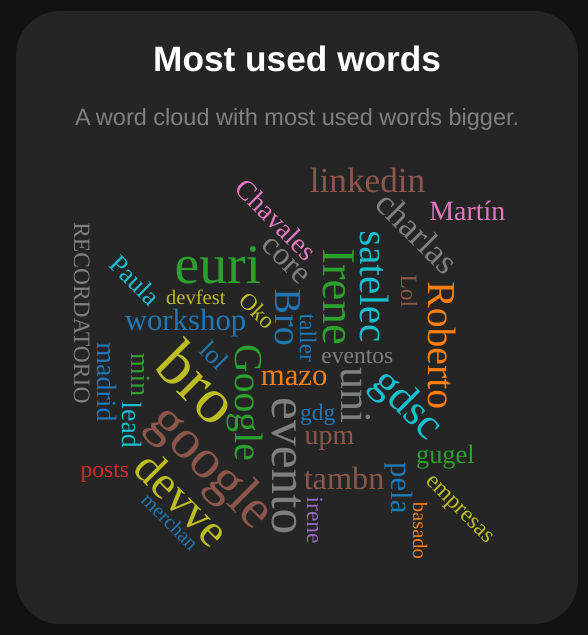
\includegraphics[width=6cm]{img/word_cloud.png} }}
	\qquad
	\subfloat[\centering Nube de emoticonos]{{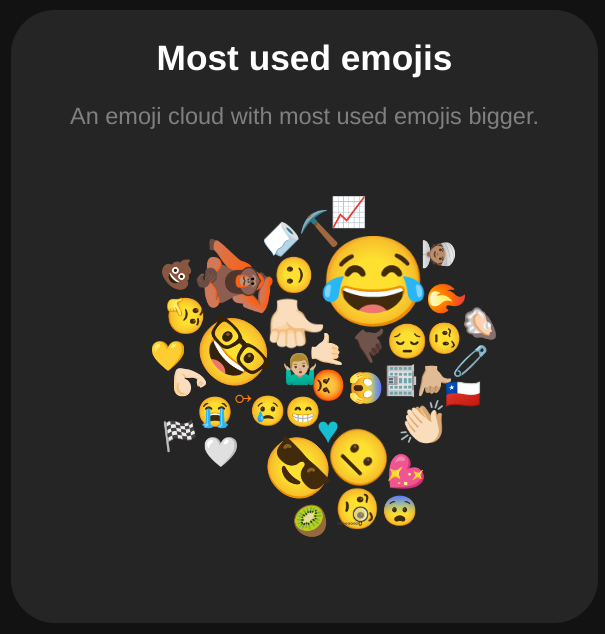
\includegraphics[width=6cm]{img/emoji_cloud.png} }}
	\caption{Nube de palabras y emoticonos}
	\label{fig:chap4:word_emoji_cloud}
\end{figure}

Se elige calcular y mostrar esta visualización puesto que los emoticonos constituyen en un chat la forma más similar a la expresión no verbal.

\subsection{Exportador}

Este módulo permite al usuario exportar tanto la visualización como exportar las métricas calculadas para su uso posterior.

\subsubsection{Compartir visualizaciones}

Compartir visualizaciones es un submódulo que, mediante el uso de la librería \textit{html2canvas} permite generar una imagen a partir de un objeto del \acrshort{dom}. Una vez generada, se crea un link falso que se pulsa por el usuario para iniciar la descarga del archivo.

\subsubsection{Exportar resultados}

Del mismo modo que el submódulo anterior, este módulo exporta las métricas obtenidas en un fichero \acrshort{json}.

\section{Conclusión}

Con todo, si en un futuro se quiere extender la arquitectura propuesta a un modelo de cliente-servidor, siempre se puede añadir un tercer contenedor en la última capa de la \autoref{chap:architecture:server} que implemente lógica adicional. Sería también necesaria cierta modificación en el código del cliente para implementar peticiones a este nuevo servicio.

